\section{Model}
\label{sec:model}

In this Section, I develop a model of fertility and housing decisions.
Households live a finite number of periods in an overlapping-generations
economy. They face persistent idiosyncratic earnings risk and transitory taste
shocks over fertility and housing. They derive utility from consumption,
housing services and children at home, and they save in a one-period bond
with an exogenous interest rate.
They either rent or own their home. Owning gives more services than renting
the same space, and the largest homes are only for sale. Owners can borrow
against their home, up to a fraction of its value, while renters cannot
borrow. A buyer must therefore make a down payment, and a seller pays a
transaction cost. During a fertile period
of their lives, households choose whether to try for a child. Children raise
the household's needs and the value of space, so the decision to have a child
is also a decision about housing. Households work until retirement and then
receive a pension, financed by a payroll tax on workers, who supply labor
inelastically. House prices and rents are determined in equilibrium.

\subsection{The economy}
\label{sec:m-env}
I begin by describing households and their preferences, the income process,
housing, the assets available for trade and the fertility process. I then
describe the housing market and firms. Time is discrete and indexed by $t$.

\subsubsection*{Households and Preferences.}
The economy is populated by overlapping generations of households, with adult
age $a=0,\dots,J$. Households can have children until age $a_F$ and work
until age $a_R$, after which they retire. A household of age $a$ survives to
age $a+1$ with probability $s_a$. Figure~\ref{fig:m-lifecycle} illustrates the
different periods of the life cycle. Households differ in wealth, housing,
labor efficiency, age and the number of children. During their fertile
years, households can choose whether to try for a child. Throughout their
life, they choose whether to rent or own their dwelling, how much housing to
demand and how much to save.
\begin{figure}[ht]
\centering
\begin{tikzpicture}[x=1.2cm,y=0.45cm,font=\small]
 \fill[blue!12] (0,0.65) rectangle (4.5,1.35); \node at (1.1,1) {fertile};
 \draw[-Latex,semithick] (2.4,1.55) to[bend left=50] node[above,inner sep=2pt] {$\pi_a$: birth} (3.4,1.55);
 \fill[green!12] (0,-0.15) rectangle (8,0.55); \node at (4,0.2) {working};
 \fill[gray!18] (8,-0.15) rectangle (11,0.55); \node at (9.5,0.2) {retired};
 \draw[thick,-Latex] (0,-0.5) -- (11.4,-0.5);
 \foreach \x/\l in {0/{$0$},4.5/{$a_F$},6/{$a$},7/{$a+1$},8/{$a_R$},11/{$J$}}
  {\draw (\x,-0.65) -- (\x,-0.35); \node[below,inner sep=2pt] at (\x,-0.65) {\l};}
 \draw[-Latex,semithick] (6,0.75) to[bend left=50] node[above,inner sep=2pt] {$s_a$} (7,0.75);
\end{tikzpicture}
\caption{Life cycle of a household. Until age $a_F$, a try for a child
succeeds with probability $\pi_a$, which declines with age. A household of age $a$ survives to age
$a+1$ with probability $s_a$.}
\label{fig:m-lifecycle}
\end{figure}

Households value consumption $c_t$, housing services $\hat h_t$ and the
number of children at home $n_t$, and discount the future by $\beta$. A
household either owns $h^O_t$ or rents $h^R_t$, and its housing services are
\begin{equation*}
 \hat h_t=\begin{cases}\chi\,h^O_t, & \text{owner},\\ h^R_t, & \text{renter},\end{cases}
 \qquad \chi>1 .
\end{equation*}
The parameter $\chi$ determines the additional services a household obtains
from owning a home of a given size. Flow utility is
\begin{equation}
 u(c_t,\hat h_t,n_t)=\frac{1}{1-\sigma}\left[\frac{c_t^{\alpha_0}\bigl(\hat h_t-\chi^{\1\{\text{own}\}}\,\bar h(n_t)\bigr)^{1-\alpha_0}}{e(n_t)}\right]^{1-\sigma}+\psi_t\,v(n_t),
 \label{eq:m-utility}
\end{equation}
with
\begin{equation*}
 \bar h(n_t)=h_P\,\1\{n_t>0\},\qquad v(n_t)=n_t^{1-\gamma}.
\end{equation*}
The first term is utility from a Cobb--Douglas composite of consumption and
housing services above a requirement $\bar h(n_t)$, per adult equivalent,
where $\alpha_0$ is the weight on consumption and $\sigma$ the curvature.
Children raise the household's needs in two ways. First, a household with
children at home must occupy $h_P$ units of housing before additional housing
yields services; an owner obtains $\chi(h^O_t-h_P)$ and a renter $h^R_t-h_P$.
The requirement does not depend on the number of children, so the first
child activates it, and the household pays for it every period its children
are at home, whether it rents or owns. Second, the equivalence scale
$e(n_t)$, with $e(0)=1$, measures adult equivalents relative to a childless
couple.\footnote{I use the scale of
\citet{scholzSeshadriKhitatrakunSaving2006},
$e(n_t)=\bigl((2+\omega n_t)/2\bigr)^{\nu}$, where $\omega$ is the weight of
a child relative to an adult and $\nu$ governs economies of scale.} The second
term, $\psi_t v(n_t)$, is the benefit of children at home: $\psi_t$ is the
preference for children and $\gamma$ governs how fast the benefit of an
additional child declines. The first child also carries a one-time utility
cost $\xi$ at birth. \textcolor{red}{[To recheck: whether the first-birth
cost $\xi$ is needed.]}

\textcolor{red}{[Check: the code applies $\chi$ to the requirement for owners, so owner services above it are $\chi(h^O_t-h_P)$, as written here; the deck's Utility Specification slide writes $\chi h^O_t-h_P$.]}

\subsubsection*{Bequests.}
A household that dies at the end of period $t$ leaves the estate
$x_{t+1}=b_{t+1}+(1-\mu)P_th^O_t$, its bond position and the value of its
home net of the selling cost. As in \citet{deNardiWealthInequality2004}, it
values the estate according to
\begin{equation*}
 B(x_{t+1})=\theta_0\,\frac{(\theta_1+x_{t+1})^{1-\sigma}}{1-\sigma},
\end{equation*}
where $\theta_0$ scales the strength of the bequest motive and $\theta_1$
determines the extent to which bequests are a luxury good. Estates are
collected by the government.

\subsubsection*{Income.}
Before retirement, a household supplies one unit of labor inelastically, with
efficiency $e_az_t$. The term $e_a$ is the age profile of earnings, and $z_t$
is idiosyncratic labor efficiency, whose logarithm follows a first-order
autoregressive process,
\begin{equation*}
 \log z_{t+1}=\rho_z\log z_t+\epsilon_{t+1},\qquad
 \epsilon_{t+1}\sim N(0,\sigma_z^2),
\end{equation*}
where $\rho_z$ is the persistence and $\sigma_z^2$ the variance of the
innovations. Earnings are taxed at rate
$\tau^w$, and retirees receive a pension $m_t$:
\begin{equation*}
 y_t(a,z_t)=\begin{cases}(1-\tau^w)\,w\,e_az_t, & a<a_R,\\ m_t, & a\ge a_R.\end{cases}
\end{equation*}
Every household also receives a transfer $T_t$, the rebate of property-tax
revenue.

\subsubsection*{Housing.}
A household enters period $t$ with the home it owned in the previous period,
$h^O_{t-1}$, which is zero for a renter. Owner-occupied homes come in a finite
set of sizes, $h^O_t\in\mathcal H$, and trade at price $P_t$ per unit of
space. Owners pay maintenance $\delta_H$ and property tax $\tau^p$ on the
value of their home, $P_th^O_t$, and selling a home costs a fraction $\mu$ of
its value. Renters choose any size up to a cap, $h^R_t\le\bar h^R$, at rent
$r_t$ per unit. Since $\bar h^R<\max\mathcal H$, the largest homes are only
for sale.

\subsubsection*{Borrowing.}
Households save or borrow in a one-period bond, traded with the rest of the
world at the exogenous gross return $R_b$. Let $b_{t+1}$ denote the bond
position a household chooses in period $t$.
Borrowing must be secured by a home, so a renter cannot borrow,
$b_{t+1}\ge0$. An owner can borrow up to a fraction $\phi$ of the current
value of its home:
\begin{equation}
 b_{t+1}\ge-\phi\,P_th^O_t .
 \label{eq:m-ltv}
\end{equation}
The limit applies both to a household that buys a home and to one that stays
in the home it owns. A buyer must therefore pay at least $(1-\phi)P_th^O_t$
itself, out of its bond position, the income of the period and the proceeds
from selling any home it owned. This down payment ties ownership, and with it
access to the largest homes, to the household's wealth. Debt is rolled over
each period at the return $R_b$: mortgages have no amortization schedule and
no limit on payments relative to income.

\subsubsection*{Fertility.}
Until age $a_F$, a household decides each period whether to try to have a
child. A try succeeds with probability $\pi_a$, which declines with age, and a
success adds one child at home in the same period. Children do not work and
make no decisions; they affect the household through its needs and through
the benefit of children in preferences. Each child at home leaves with
probability $\lambda$ per period, independently of its siblings, so a child
stays at home for $1/\lambda$ periods on average. Children who leave form new
households and enter the economy at age $0$, with an initial wealth position
drawn from an exogenous distribution.

\subsubsection*{Housing supply.}
Housing is built by absentee developers, who sell it to households and to
landlords at the price $P_t$ per unit. I do not model the construction
technology explicitly. Instead, the aggregate housing stock is an increasing
function of the current price,
\begin{equation}
 H_t=H_0\,P_t^{\eta},
 \label{eq:m-supply}
\end{equation}
where $H_0>0$ sets the scale of the stock and $\eta\ge0$ is the price
elasticity of housing supply. The stock in period $t$ depends only on the
price in period $t$, so supply adjusts within the period. The elasticity
governs how a change in the demand for housing is split between the price and
the quantity. When $\eta=0$ the stock is fixed and the price absorbs the whole
change; the larger is $\eta$, the more the stock adjusts and the less the
price moves. The stock is divided between owner-occupied and rental housing
by households' tenure choices.

\subsubsection*{Rental market.}
A household that does not own a home rents from landlords. Landlords are
competitive and owned by agents outside the economy. A landlord buys housing
at the price $P_t$, rents it to households at the rent $r_t$ per unit, pays
maintenance and property tax on its value, $(\delta_H+\tau^p)P_t$, and sells
it at the price $P_{t+1}$ in the next period. Landlords finance their
purchases at the gross return $R_b$ and, unlike households, pay no
transaction cost when they sell. Competition drives their profit to zero, so
the return on a unit of rental housing equals the return on the bond:
\begin{equation}
 r_t+P_{t+1}-(\delta_H+\tau^p)P_t=R_b\,P_t .
 \label{eq:m-rent}
\end{equation}
Landlords supply any quantity of rental housing at this rent. Rearranging,
\begin{equation*}
 r_t=(R_b-1+\delta_H+\tau^p)\,P_t-(P_{t+1}-P_t).
\end{equation*}
The rent equals the user cost of housing: the interest forgone on the price,
plus maintenance and property tax, net of the capital gain. The rent
therefore depends on the expected path of the price, not only on its current
level. When the price is expected to fall, the rent rises relative to the
price, because landlords must be compensated for the expected capital loss. \textcolor{red}{[To review: written as on the slides and in the production
code. How maintenance and the rent are accounted for, for owners and for
landlords, is under review (accounting test, Oct 17).]}

\subsubsection*{Firms.}
A representative firm produces the consumption good, which is the numeraire,
with a linear technology in effective labor,
\begin{equation*}
 Y_t=A\,L_t,\qquad L_t=\int_{a<a_R}e_az_t\,\dd G_t,
\end{equation*}
where $A$ is productivity, $G_t$ is the measure of households over states and
$L_t$ is the total efficiency units of labor supplied by households of working
age. The firm is competitive and pays each efficiency unit its marginal
product, $w=A$. The wage is therefore constant over time.

\subsubsection*{Government.}
The government runs a pay-as-you-go pension system, taxes housing and collects
estates. It taxes
earnings at the constant rate $\tau^w$ and pays the same pension $m_t$ to
every retired household. The pension system balances its budget every period,
so the pension equals payroll-tax revenue divided by the number of retired
households. When the number of retirees rises relative to effective labor, the
pension falls. The government also levies the property tax $\tau^p$ on the
value of all housing, owned and rented, and returns the revenue to households
as a lump-sum transfer $T_t$, equal across households. Finally, the government
collects the estates of the households that die. It uses them to pay new
households their initial wealth and spends the remainder on government
consumption, which does not affect households.

\subsection{The household's problem}
\label{sec:m-household}

I next characterize the household's problem recursively. A period has two
stages, shown in Figure~\ref{fig:m-timing}. At the beginning of the period,
the household observes its fertility taste shocks and decides whether to try
for a child. After the birth outcome, it observes its housing taste shocks and
chooses its home and saving. A birth therefore changes the demand for housing
in the same period. The state of a household is its bond position $b_t$, the
home it owns $h^O_{t-1}$, its efficiency $z_t$, its age $a_t$ and the number of
children at home $n_t$.

\begin{figure}[ht]
\centering
\begin{tikzpicture}[node distance=5mm and 6mm, >=Latex, font=\small,
 see/.style={ellipse, draw, fill=yellow!20, minimum height=1.4em, inner sep=2pt, align=center},
 choose/.style={rectangle, draw, fill=green!15, rounded corners=2pt, minimum height=1.6em, inner sep=3pt, align=center},
 line/.style={-Latex, semithick}]
\node (vt) {$V_t$};
\node (fertS) [see, right=4mm of vt] {see $\varepsilon^F_t$};
\node (fertD) [choose, right=of fertS] {try or not};
\node (vh) [right=12mm of fertD] {$V^H_t$};
\node (locS) [see, right=4mm of vh] {see $\varepsilon^H_t$};
\node (locD) [choose, right=of locS] {choose $h^O_t,h^R_t,b_{t+1}$};
\draw[line] (vt) -- (fertS);
\draw[line] (fertS) -- (fertD);
\draw[line] (fertD) -- node[above]{birth} (vh);
\draw[line] (vh) -- (locS);
\draw[line] (locS) -- (locD);
\end{tikzpicture}
\caption{Timing within period $t$.}
\label{fig:m-timing}
\end{figure}

\subsubsection*{Fertility.}
Let $V_t(b_t,h^O_{t-1},z_t,a_t,n_t)$ denote the value of a household at the
beginning of period $t$, before it observes its fertility shocks. A household
of fertile age chooses between not trying, $j=0$, and trying, $j=A$. Each
option receives a taste shock
$\varepsilon^F_{t,j}\overset{iid}{\sim}\text{Gumbel}(0,\kappa)$, with
$\kappa=\kappa_1$ before the first child and $\kappa=\kappa_C$ after. The
separate scales allow the decision to become a parent to respond differently
from the decision to have another child. The value of the household and the
probability of trying are
\begin{equation}
\begin{aligned}
 V_t&=\E_{\varepsilon^F_{t,j}}\max_{j\in\{0,A\}}\bigl\{V^F_{t,j}+\varepsilon^F_{t,j}\bigr\}
 =\kappa\log\bigl[\exp\bigl(V^F_{t,0}/\kappa\bigr)+\exp\bigl(V^F_{t,A}/\kappa\bigr)\bigr],\\
 \pi^F_{t,a}&=\frac{\exp\bigl(V^F_{t,A}/\kappa\bigr)}{\exp\bigl(V^F_{t,0}/\kappa\bigr)+\exp\bigl(V^F_{t,A}/\kappa\bigr)},
\end{aligned}
 \label{eq:m-fertility}
\end{equation}
where $V^F_{t,0}$ and $V^F_{t,A}$ are the values of not trying and trying
before the shocks. Both depend on $V^H_t$, the value of the household after the
birth outcome, which I define below:
\begin{equation*}
\begin{aligned}
 V^F_{t,0}&=V^H_t(b_t,h^O_{t-1},z_t,a_t,n_t),\\
 V^F_{t,A}&=\pi_a\bigl[V^H_t(b_t,h^O_{t-1},z_t,a_t,n_t+1)-\xi\,\1\{\text{first child}\}\bigr]+(1-\pi_a)\,V^F_{t,0}.
\end{aligned}
\end{equation*}
Not trying leaves the number of children at home unchanged. Trying succeeds
with probability $\pi_a$, adds a child at home and, for the first child,
carries the utility cost $\xi$; if it fails, the household is in the same
position as if it had not tried. Given its state, a household has a child
with probability $\pi_a\pi^F_{t,a}$. Outside the fertile ages, there is no
fertility choice and $V_t=V^H_t(b_t,h^O_{t-1},z_t,a_t,n_t)$.

\subsubsection*{Housing and savings.}
After the birth outcome, the household observes its housing taste shocks and
chooses its home, its tenure and its bond position. Let $n_{t+1}$ denote the
number of children at home after this period's birth outcome. Before the
housing shocks, the value of the household is
\begin{multline}
 V^H_t(b_t,h^O_{t-1},z_t,a_t,n_{t+1})
 =\E_{\varepsilon^H_{t,j}}\max_{h^O_t,h^R_t,b_{t+1}}
 \Bigl\{u(c_t,\hat h_t,n_{t+1})+\varepsilon^H_{t,j}\\
 +\beta\,\E_t\Bigl[s_aV_{t+1}(b_{t+1},h^O_t,z_{t+1},a_t+1,n_{t+1})
 +(1-s_a)B(x_{t+1})\Bigr]\Bigr\},
 \label{eq:m-vh}
\end{multline}
subject to the budget constraint of the chosen option,
\begin{equation}
\begin{aligned}
 &\text{Buy:}  && c_t+b_{t+1}+(\delta_H+\tau^p)P_th^O_t=R_bb_t+y_t+T_t-P_t\bigl[h^O_t-(1-\mu)h^O_{t-1}\bigr],\\
 &\text{Stay:} && c_t+b_{t+1}+(\delta_H+\tau^p)P_th^O_t=R_bb_t+y_t+T_t,\\
 &\text{Rent:} && c_t+b_{t+1}+r_th^R_t=R_bb_t+y_t+T_t+(1-\mu)P_th^O_{t-1},
\end{aligned}
 \label{eq:m-budget}
\end{equation}
and the borrowing limit \eqref{eq:m-ltv} for buyers and stayers, or
$b_{t+1}\ge0$ for renters. A buyer sells the home it owns, if any, and buys a
new one; a stayer keeps its home; a renter sells the home it owns, if any, and
rents. The expectation $\E_t$ is over next period's efficiency and the
departure of children. The shocks
$\varepsilon^H_{t,j}\overset{iid}{\sim}\text{Gumbel}(0,\kappa_T)$ are one per
option $j$: renting, or owning each $h^O\in\mathcal H$. Let $V^j_t$ denote the
value of option $j$ before the shock. Then
\begin{equation}
 V^H_t=\kappa_T\log\sum_{j}\exp\bigl(V^j_t/\kappa_T\bigr),
 \qquad
 \pi^H_t(j)=\frac{\exp(V^j_t/\kappa_T)}{\sum_{j'}\exp(V^{j'}_t/\kappa_T)},
 \label{eq:m-tenure}
\end{equation}
where $\pi^H_t(j)$ is the probability of choosing option $j$. \textcolor{red}{[To consider: dropping the
tenure taste shocks $\varepsilon^H_{t,j}$.]} An option that
leaves no saving choice within the budget and borrowing constraints cannot be
chosen. Housing costs, credit and earnings risk shape $V^H_t$, and through it
the gap $V^F_{t,A}-V^F_{t,0}$ that governs fertility.

\subsection{Equilibrium}
\label{sec:m-equilibrium}

\textcolor{red}{[To review: the equilibrium definition.]}

\begin{definition}
Given an initial measure of households over states $G_0$, an equilibrium is
a path of prices $\{P_t,r_t\}$, pensions $\{m_t\}$, rebates $\{T_t\}$, value
and policy functions, and measures $\{G_t\}$ consistent with the policy
functions, the shocks, survival and entry, such that every period:
\begin{enumerate}
\item \emph{Households} solve their problem, given prices, transfers and
shocks, and rent satisfies the landlords' zero-profit condition
\eqref{eq:m-rent}.
\item \emph{Housing market} clears: owned and rented housing equal the stock,
\[
 \int\bigl(h^O_t+h^R_t\bigr)\,\dd G_t=H_t .
\]
\item \emph{Pensions}: payroll taxes pay the pensions of the $N^R_t$ retired
households, $\tau^wwL_t=m_tN^R_t$.
\item \emph{Rebate}: property-tax revenue is paid to all $N_t$ households,
$T_tN_t=\tau^pP_t\int\bigl(h^O_t+h^R_t\bigr)\,\dd G_t$.
\item \emph{Population}: births are $B_t=\int\pi_a\pi^F_{t,a}\,\dd G_t$, and
new households are $E_t=\lambda K_t$, where $K_t$ is the number of children
at home.
\end{enumerate}
\end{definition}

\begin{definition}
A stationary equilibrium is a price $P$, a rent $r$, a pension $m$, a rebate
$T$, value and policy functions, and a measure of households over states
$G$, such that:
\begin{enumerate}
\item \emph{Households} solve their problem, given $P$, $r$, $m$ and $T$.
\item \emph{Rent} satisfies the landlords' zero-profit condition at a
constant price, $r=(R_b-1+\delta_H+\tau^p)P$.
\item \emph{Housing market} clears,
$\int\bigl(h^O+h^R\bigr)\,\dd G=H_0P^{\eta}$.
\item \emph{Pensions and rebate} balance, $\tau^wwL=mN^R$ and
$TN=\tau^pP\int\bigl(h^O+h^R\bigr)\,\dd G$.
\item \emph{The measure $G$ is invariant}: the policy functions, the shocks,
survival and the entry of $E=\lambda K$ new households map $G$ into itself.
\end{enumerate}
\end{definition}

\subsection{Model analysis}
\label{sec:m-analysis}

Three tensions shape fertility in the model. The first is timing: the chance
of a birth falls with age, while earnings and wealth rise, and owning the
space a child needs takes a down payment. The second is risk: the child's
space is paid for in every period the child is at home, out of uncertain
earnings. The third runs through the housing market: fewer children lower the
demand for housing and its price, and a lower price raises fertility.
Section~\ref{sec:results} measures the cost of the child's space and the role
of risk, Section~\ref{sec:policy-credit} the role of the down payment, and
Section~\ref{sec:quant-transition} the response of the housing market.

\subsubsection*{Borrowing limits and the timing of children.}
A try for a child succeeds with probability $\pi_a$, which declines with age,
while earnings $e_az_t$ rise with age through $e_a$
(Figure~\ref{fig:m-agetiming}a). A child raises by $r_th_P$ the spending
needed for the same housing services, in every period it is at home. The home
a family wants also requires a down payment: a renter cannot borrow, and an
owner can borrow only against its home. Let $\zeta_t\ge0$ denote the
multiplier on the borrowing limit, $b_{t+1}\ge-\phi P_th^O_t$ with $h^O_t=0$
for a renter: the value, in utility, of borrowing one more unit in period
$t$.\footnote{Appendix~\ref{app:household} derives the Euler equation for the
bond and the conditions behind the results below.} A birth raises the
multiplier when it raises marginal utility more today than next period, as
for a household whose earnings rise. Such a household can delay the child, at
the cost of a lower $\pi_a$. It can have the child in rented space and forgo
$\chi$ and the homes larger than $\bar h^R$. Or it can have the child and buy
once its savings cover the down payment.

\begin{figure}[ht]
\centering
\begin{tikzpicture}[>=Latex,font=\small]
\begin{scope}[x=0.62cm,y=0.62cm]
 \fill[blue!8] (0,0) rectangle (4.5,5.2);
 \node[text=blue!60!black] at (2.25,0.45) {fertile};
 \draw[->,semithick] (0,0) -- (10.6,0) node[below left] {age $a$};
 \draw[->,semithick] (0,0) -- (0,5.6);
 \draw[very thick,blue!60!black] (0,4.2) .. controls (2.2,4.1) and (3.6,3.5) .. (4.5,2.3);
 \draw[blue!60!black,densely dotted] (4.5,2.3) -- (4.5,0);
 \node[text=blue!60!black,anchor=south west] at (1.4,4.15) {$\pi_a$};
 \draw[very thick,orange!80!black] (0,1.0) .. controls (2.5,1.6) and (5,3.4) .. (8,3.6);
 \node[text=orange!80!black,anchor=south] at (7.4,3.7) {$e_a$};
 \draw[densely dashed,gray] (8,0) -- (8,3.6);
 \foreach \x/\l in {0/{$0$},4.5/{$a_F$},8/{$a_R$}}
  {\draw (\x,0.08) -- (\x,-0.08); \node[below] at (\x,-0.08) {\l};}
 \node[align=center] at (5.1,-1.5) {(a) Fertility declines with age,\\ earnings rise};
\end{scope}
\begin{scope}[xshift=7.9cm,x=0.62cm,y=0.62cm]
 \fill[blue!8] (0,0) rectangle (4.5,5.2);
 \draw[->,semithick] (0,0) -- (10.6,0) node[below left] {age $a$};
 \draw[->,semithick] (0,0) -- (0,5.6) node[above right] {housing $h$};
 \draw[densely dotted,gray] (0,2.6) -- (10,2.6); \node[left] at (0,2.6) {$\bar h^R$};
 \draw[densely dotted,gray] (2.2,0) -- (2.2,4.6); \node[anchor=south,font=\footnotesize] at (2.2,4.6) {birth};
 \draw[very thick,mechnavy] (0,1.5) -- (2.2,1.5) -- (2.2,2.6) -- (3.53,2.6);
 \draw[very thick,mechnavy] (3.53,2.6) -- (6.86,2.6) -- (6.86,4.2) -- (10,4.2);
 \draw[very thick,mechteal,densely dashed] (3.53,2.6) -- (3.53,4.2) -- (6.86,4.2);
 \fill[mechteal,opacity=0.15] (3.53,2.6) rectangle (6.86,4.2);
 \node[text=mechnavy,anchor=south] at (8.5,4.2) {$h^O$};
 \node[text=mechnavy,anchor=north,font=\footnotesize,align=center] at (5.2,2.45) {rents at\\ the cap};
 \draw[->,mechteal] (6.75,0.45) -- (3.65,0.45);
 \draw[mechnavy,densely dotted] (6.86,2.6) -- (6.86,0);
 \draw[mechteal,densely dotted] (3.53,2.6) -- (3.53,0);
 \foreach \x/\l in {0/{$0$},4.5/{$a_F$}}
  {\draw (\x,0.08) -- (\x,-0.08); \node[below] at (\x,-0.08) {\l};}
 \node[text=mechnavy,anchor=west,font=\footnotesize] at (7.1,3.4) {$\phi$};
 \node[text=mechteal,anchor=east,font=\footnotesize] at (3.4,3.4) {$\phi'$};
 \node[align=center] at (5.1,-1.5) {(b) A higher $\phi'>\phi$ brings\\ family space forward};
\end{scope}
\end{tikzpicture}
\caption{Timing of fertility, earnings and the purchase of a family home}
\label{fig:m-agetiming}
\par\smallskip
\begin{minipage}{0.92\linewidth}
\footnotesize\textit{Notes:} Schematic. The shaded area marks the fertile
ages. In panel (b), the solid line is the housing of a household that rents
until its savings cover the down payment on a family home $h^O$ at the
loan-to-value ratio $\phi$. The dashed line is the same household at
$\phi'>\phi$, and the shaded area is the family space it gains.
\end{minipage}
\end{figure}

A higher loan-to-value ratio $\phi$ lowers the equity $(1-\phi)P_th^O_t$ a
buyer needs and allows an earlier purchase (Figure~\ref{fig:m-agetiming}b).
It leaves the cost of a child's space unchanged: by \eqref{eq:m-rent}, that
space costs about $r_th_P$ every period, whether the household rents or
owns.\footnote{Apart from the selling cost, an owner that holds a unit from
$t$ to $t+1$ pays $(1+\tau^p)P_t$ in period $t$ and holds $(1-\delta_H)P_{t+1}$
in period $t+1$, so by \eqref{eq:m-rent} its cost, in period-$t$ units, equals
the rent $r_t$.} For a change in $\phi$ in period $t$, the envelope theorem,
\eqref{eq:m-tenure} and \eqref{eq:m-fertility} give\footnote{Here
$\kappa=\kappa_1$ before the first child and $\kappa_C$ after. A permanent
change in $\phi$ adds the corresponding terms for all future periods,
discounted and weighted by survival.}
\begin{equation}
 \begin{gathered}
 \frac{\partial\pi^F_{t,a}}{\partial\phi}
 =\frac{\pi^F_{t,a}\bigl(1-\pi^F_{t,a}\bigr)}{\kappa}\;\pi_a
 \left[\frac{\partial V^H_t(n_t+1)}{\partial\phi}-\frac{\partial V^H_t(n_t)}{\partial\phi}\right],
 \\
 \frac{\partial V^H_t(n)}{\partial\phi}
 =\sum_{h^O\in\mathcal H}\pi^H_t(h^O\mid n)\,\zeta_t(h^O,n)\,P_th^O ,
 \end{gathered}
 \label{eq:m-credit}
\end{equation}
where $\pi^H_t(h^O\mid n)$ is the probability of owning $h^O$ and
$\zeta_t(h^O,n)$ the multiplier in that option. The second line is the value
of credit to a household with $n$ children at home: an owner of $h^O$ can
borrow $P_th^O$ more, and each unit is worth $\zeta_t(h^O,n)$. Credit is worth
nothing to a household that rents or whose limit is slack. The first line
says that credit raises the probability of trying only through the difference
between its value with the additional child and without it. The difference is
positive when the child moves the household toward larger owned homes, where
the limit binds, close to zero for a household that rents either way, and
negative when credit mainly helps households without children to buy. The
factor in front is largest for households close to indifferent about trying
and falls with age through $\pi_a$. Section~\ref{sec:policy-credit} shows
which case dominates in the calibrated model: credit mostly lets young
households buy the small homes they would otherwise rent, and it brings
births forward.

\subsubsection*{Earnings risk.}
A child stays at home for $1/\lambda$ periods on average, while earnings are
risky and persistent. Consider a renter at the borrowing limit,
$b_t=b_{t+1}=0$, that rents below the cap. Maximizing \eqref{eq:m-utility}
subject to $c_t+r_th^R_t=y_t+T_t$ gives the flow utility
\begin{equation}
 u(c_t,h^R_t,n_t)=\frac{1}{1-\sigma}\left[\frac{\alpha_0^{\alpha_0}(1-\alpha_0)^{1-\alpha_0}}{r_t^{1-\alpha_0}}\;
 \frac{y_t+T_t-r_t\bar h(n_t)}{e(n_t)}\right]^{1-\sigma}+\psi_t\,v(n_t).
 \label{eq:m-indirect}
\end{equation}
The child's space is a committed expenditure, paid out of income before the
household divides the rest between consumption and additional space. Let
$\Delta_t(y_t)$ be the utility cost of a first child: the first term of
\eqref{eq:m-indirect} with $n_t=0$ minus the same term with $n_t=1$. For
$\sigma\ge1$, $\Delta_t$ is decreasing and convex in earnings, and more convex
when $r_th_P$ is larger.\footnote{Let $\tilde y_t=y_t+T_t$, $k=r_th_P$ and
$\Theta_t=\alpha_0^{\alpha_0}(1-\alpha_0)^{1-\alpha_0}r_t^{\alpha_0-1}$. Then
$\Delta_t''(\tilde y_t)=\sigma\Theta_t^{1-\sigma}\bigl[e(1)^{\sigma-1}(\tilde y_t-k)^{-\sigma-1}-\tilde y_t^{-\sigma-1}\bigr]$,
which is positive for $\sigma\ge1$, since $e(1)\ge1$ and $k>0$, and rises
with $k$.} By Jensen's inequality, earnings risk raises the expected cost of a
child above its cost at expected earnings, and by more when the child's space
is more expensive (Figure~\ref{fig:m-risk}). Savings soften this effect.
Section~\ref{sec:results-risk} measures it in the calibrated model.

\begin{figure}[ht]
\centering
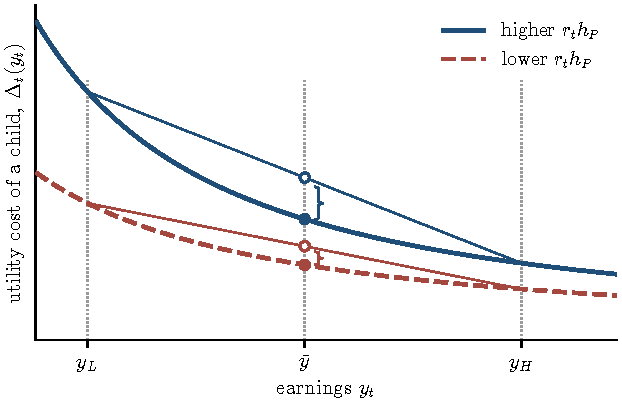
\includegraphics[width=0.65\textwidth]{figures/fig_m_risk_fi.pdf}
\caption{Earnings risk and the utility cost of a child}
\label{fig:m-risk}
\par\smallskip
\begin{minipage}{0.92\linewidth}
\footnotesize\textit{Notes:} The figure is computed from \eqref{eq:m-indirect} at the
parameters of Section~\ref{sec:quant} (Appendix~\ref{app:model-figures}).
The curves plot $\Delta_t$ for a renter at the borrowing limit, at the rent of
the initial steady state (solid) and at the rent of the new steady state of
Figure~\ref{fig:m-illustration} (dashed). Earnings are $y_L$ or $y_H$ with
equal probability. Filled circles mark the cost at expected earnings $\bar y$
and open circles the expected cost; the braces mark the additional cost due to
risk.
\end{minipage}
\end{figure}

\subsubsection*{Households and the housing market.}
Figure~\ref{fig:m-illustration} shows how the economy responds to a fall in
the preference for children, from $\psi_0$ to $\psi_1$. Panel (a) shows the
housing market in a steady state. Supply \eqref{eq:m-supply} rises with the
price. Demand, $N\,h(P;\psi)$, is the number of households $N$ times the
housing each one owns or rents at the price $P$.\footnote{In a steady state,
the housing market (Section~\ref{sec:m-equilibrium}) clears when this demand equals the stock.
Housing and fertility respond to the rent. In a steady state, the rent is
proportional to the price by \eqref{eq:m-rent}, so both can be read against
the price. Along a transition, the rent also reflects the expected change in
the price.} Panel (b) shows the fertility $n(P;\psi)$ that households choose
at each price. At $A$, the market clears at $P_0$ with $N_0$ households, and
fertility is at the replacement rate $\bar n$. When the preference falls, the
population is inherited and the price stays close to $P_0$, so fertility
falls along $n(P;\psi_1)$, from $A$ to $A'$. Over the following generations,
smaller cohorts reduce the number of households, demand shifts left, and the
price falls along the supply curve. The lower price raises fertility along
$n(P;\psi_1)$, until fertility is back at replacement at $B$, with fewer
households and cheaper housing. The transition of
Section~\ref{sec:quant-transition} follows these steps.

In a steady state, the number of new households equals the number that die,
so fertility is at the replacement rate. Since the household problem, the
pension and the rebate per household do not depend on the number of
households, the condition $n(P;\psi)=\bar n$ in panel (b) determines the
steady-state price, and supply and demand in panel (a) then determine the
number of households. A more elastic supply therefore leaves the steady-state
price unchanged and implies a larger fall in the number of households.

\begin{figure}[ht]
\centering
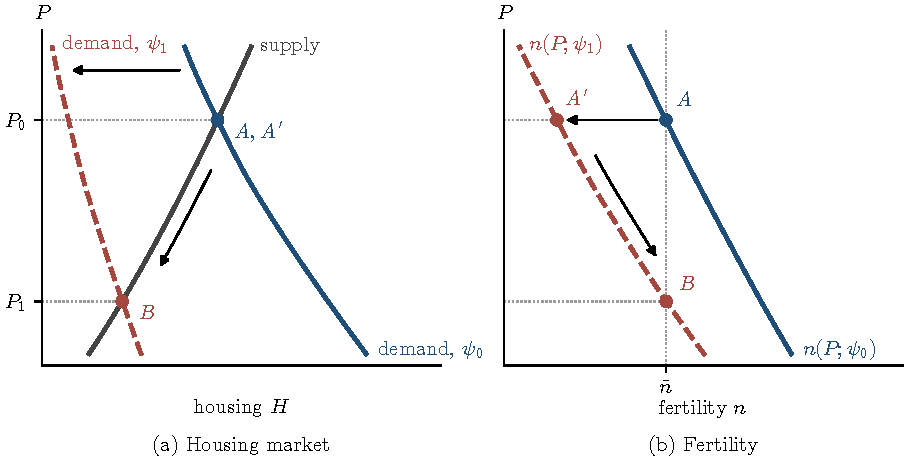
\includegraphics[width=\textwidth]{figures/fig_m_illustration_demand.pdf}
\caption{The housing market and fertility}
\label{fig:m-illustration}
\par\smallskip
\begin{minipage}{0.92\linewidth}
\footnotesize\textit{Notes:} The figure is computed from stationary solves of
the model at given prices, at the parameters of Section~\ref{sec:quant}
(Appendix~\ref{app:model-figures}). Panel (a) shows housing supply
\eqref{eq:m-supply} and demand with $N_0$ households under $\psi_0$ (solid)
and $N_1$ households under $\psi_1$ (dashed). Panel (b) shows the fertility
households choose at each price; the dotted line marks replacement. $A$ is the
initial steady state, $A'$ the outcome at the inherited population after the
fall in $\psi$, and $B$ the new steady state.
\end{minipage}
\end{figure}
